\documentclass[a4paper, 11pt]{article}

\usepackage[left=1.5cm, right=1.5cm, top=2cm, bottom=2cm]{geometry}

\usepackage[utf8]{inputenc}
\usepackage[T1]{fontenc}
\usepackage[english]{babel}  
\usepackage{lmodern}

\usepackage{amsmath, amsthm, amssymb}
\usepackage{mathtools}
\usepackage{booktabs}
\usepackage{stmaryrd}

\usepackage{wrapfig}

\usepackage{tikz}
\newcommand{\boxalign}[2][0.97\textwidth]
{\par\noindent\tikzstyle{mybox} = [draw=black,inner sep=6pt]
  \begin{center}\begin{tikzpicture}
   \node [mybox] (box){%
    \begin{minipage}{#1}{\vspace{-5mm}#2}\end{minipage}
   };
  \end{tikzpicture}
  \end{center}}

\newtheorem{innercustomgeneric}{\customgenericname}
\providecommand{\customgenericname}{}
\newcommand{\newcustomtheorem}[2]{%
  \newenvironment{#1}[1]
  {%
   \renewcommand\customgenericname{#2}%
   \renewcommand\theinnercustomgeneric{##1}%
   \innercustomgeneric}
  {\endinnercustomgeneric}
}

\newcustomtheorem{thm}{Theorem}
\newcustomtheorem{lem}{Lemma}
\newcustomtheorem{cor}{Corollary}
\newcustomtheorem{deftn}{Definition}
\newcustomtheorem{prop}{Proposition}
\DeclareMathOperator*{\argmin}{argmin} 
\DeclareMathOperator*{\argmax}{argmax} 

\begin{document}
\title{Estimation of the twist vector}
\author{Yoann Pradat}
\maketitle
\tableofcontents
\clearpage

\section{Estimation of twist vector at corners of a single patch}

Suppose we would like to represent a surface over the patch ${[0,1]}^2$ from data at each of the 4 corners.  Depending 
on the available data, different interpolation techniques (with different properties) can be used. In case of bicubic 
polynomial interpolation (“bicubic patch”) one can represent a surface from knowledge of coordinates of the surface 
value and it's first-order derivatives (that is 16 vectors in total) as $\sigma : {[0,1]}^2 \to \mathbb{R}^3$ given by

\begin{equation}
  \sigma(u,v) = \begin{bmatrix} f_1(u) \\ f_1(1-u) \\ f_2(u) \\ -f_2(1-u) \end{bmatrix}^T
  \begin{bmatrix}
    \sigma(0,0) & \sigma(0,1) & \sigma_2(0,0) & \sigma_2(0,1) \\
    \sigma(1,0) & \sigma(1,1) & \sigma_2(1,0) & \sigma_2(1,1) \\
    \sigma_1(0,0) & \sigma_1(0,1) & \sigma_{12}(0,0) & \sigma_{12}(0,1) \\
    \sigma_1(1,0) & \sigma_1(1,1) & \sigma_{12}(1,0) & \sigma_{12}(1,1) \\
  \end{bmatrix}
  \begin{bmatrix} f_1(v) \\ f_1(1-v) \\ f_2(v) \\ -f_2(1-v) \end{bmatrix}
\end{equation}

With $f_1$ and $f_2$ being the cubic Hermite polynomials over $[0,1]$
\begin{align*}
  f_1(u) &= 1 - 3u^2 + 2u^3 \\
  f_2(u) &= u - 2u^2 + u^3 \\
\end{align*}

The parameters $\sigma_{12}$ are the cross-derivatives according to each direction and as such do not lend itself to a 
consistent interpretation.  As a consequence, techniques have been developed to estimate the “optimal” twist vector with 
different optimality criterions. 

\subsection{Selesnick's method}

In his paper of 1980 Selesnick proposes to estimate separately the normal and tangential component of the twist vector 
\textbf{from the rest of the parameters and the Gaussian curvature $K$.} \\

Let's denote $n = \sigma_1 \land \sigma_2$ the normal vector and $\hat{n} = \frac{n}{|n|}$ it's normalized version. As 
for the surface with denote we subscript 1 and 2 the derivative with respect to $u$ and $v$ in that order. Then the 
normal component of the twist vector can be obtained from

\begin{equation}
  \hat{n}.\sigma_{12} = \pm \sqrt{\hat{n}.\sigma_{11} \hat{n}.\sigma_{22} - K\left(\sigma_1^2 \sigma_2^2 - 
  \sigma_1.\sigma_2 \right)}
\end{equation}

How to get the values for $\sigma_{11}, \sigma_{22}$? Supposing $\sigma, \sigma_1, \sigma_2$ are known at the corners, 
one can readily compute the values of $\sigma_{11}$ and $\sigma_{22}$. This is a consequence of having interpolators 
that are \emph{twice differentiable} and \emph{satisfy Hermite interpolation properties} that is to say

\begin{equation}
  f_1(\nu) = \delta_{\nu} \quad f_1^{(1)}(\nu) = 0 \quad f_2(\nu) = 0 \quad f_2^{(1)}(\nu) = \delta_{\nu}
\end{equation}

as the terms corresponding to the twist vectors will appear with factor $f_2^{(2)}(u)f_2(v)$, which is equal to 0 when 
$u$ and $v$ are 0 or 1. Knowing all quantities on the right-hand side of the equation above, we can estimate the normal 
component of the twist vector. As for the sign, one can choose say positive sign for the first corner and deduce the 
signs for all other corners under the assumption that the variation of the interpolated surface between the data points 
should less than the variation implied by the points themselves.\\

To get a complete description of the twist vector it is enough to compute projection of the vector on two additional 
vectors that are each orthogonal to the normal and between themselves. One is naturally led towards computing tangential 
components of the twist vector that is $\sigma_1.\sigma_{12}$ and $\sigma_2.\sigma_{12}$. Introducing the 
parametrisation by arclength $s$ for say $u$ at fixed $v$, it is straightforward to show that

\begin{equation}
  \sigma_1.\sigma_{12} = \left[\frac{ds}{du}\right] \frac{\partial}{\partial v} \left[\frac{ds}{du}\right]
\end{equation}

with $\frac{ds}{du} = |\sigma_1|$.

In a similar fashion the other tangential component is obtained by

\begin{equation}
  \sigma_2.\sigma_{12} = \left[\frac{ds}{dv}\right] \frac{\partial}{\partial u} \left[\frac{ds}{dv}\right]
\end{equation}

with $\frac{ds}{du} = |\sigma_2|$.

\subsection{Minimum quadratic oscillation}

A piecewise Coon's surface is described on a square $[a, b]\times[c,d]$ by $M_1 \times M_2$ patches of the form $I_{k,l} 
= [u_{k}, u_{k+1}]\times[v_l, v_{l+1}]$. \\

In case of a \emph{bilinear interpolating patch}, the surface on $I_{k,l}$ is given by

\begin{equation}
  \sigma(u,v) = \begin{bmatrix} f_1(u) \\ f_1(1-u)  \end{bmatrix}^T
  \begin{bmatrix}
    \sigma(0,0) & \sigma(0,1) \\
    \sigma(1,0) & \sigma(1,1) \\
  \end{bmatrix}
  \begin{bmatrix} f_1(v) \\ f_1(1-v) \end{bmatrix}
\end{equation}

wiht $f_1(u) = u$. \\

In case of \emph{bicubic Coon's patch}, the surface on $I_{k,l}$ is given by

\begin{equation}
  \sigma(u,v) = \begin{bmatrix} f_1(u) \\ f_1(1-u) \\ f_2(u) \\ -f_2(1-u) \end{bmatrix}^T
  \begin{bmatrix}
    \sigma(0,0) & \sigma(0,1) & \sigma_2(0,0) & \sigma_2(0,1) \\
    \sigma(1,0) & \sigma(1,1) & \sigma_2(1,0) & \sigma_2(1,1) \\
    \sigma_1(0,0) & \sigma_1(0,1) & \sigma_{12}(0,0) & \sigma_{12}(0,1) \\
    \sigma_1(1,0) & \sigma_1(1,1) & \sigma_{12}(1,0) & \sigma_{12}(1,1) \\
  \end{bmatrix}
  \begin{bmatrix} f_1(v) \\ f_1(1-v) \\  f_2(v) \\ - f_2(1-v) \end{bmatrix}
\end{equation}


with renoting $u \leftarrow \frac{u-u_k}{\Delta u_k}$, $v \leftarrow \frac{v-v_l}{\Delta v_l}$, $\sigma(u,v) \leftarrow 
\sigma(\frac{u-u_k}{\Delta u_k}, \frac{v-v_l}{\Delta v_l})$ and $f_1$ and $f_2$ being the cubic Hermite polynomials over 
$[0,1]$
\begin{align*}
  f_1(u) &= 1 - 3u^2 + 2u^3 \\
  f_2(u) &= u - 2u^2 + u^3 \\
\end{align*}

\underline{Remark} Renoting $\sigma(u,v) \leftarrow \sigma(\frac{u-u_k}{\Delta u_k}, \frac{v-v_l}{\Delta v_l})$ means we 
note again $\sigma$ the function on ${[0,1]}^2$ that is equal to $\sigma$ on $I_{k,l}$ mapped to ${[0,1]}^2$ that is 
$\sigma(u,v) = \sigma(\Delta u_k u + u_k, \Delta v_l v + v_l)$. As a consequence, $\sigma_1(0,0)$ in new notation 
corresponds to $ \Delta u_k \sigma_1(u_k, v_l)$ in old notation. In coherence with previous usage we would write 
$\sigma_1(u,v) \leftarrow \Delta u_k \sigma_1(\frac{u-u_k}{\Delta u_k}, \frac{v-v_l}{\Delta v_l})$.  \\ 

In their paper of 2017, X. Guo et X. Han derives a method to determine twist vectors that are optimal in the sense that 
they minimize the quadratic oscillation in average that is to say they minimize the distance between the bicubic and 
bilinear interpolant

\begin{equation}
  \int_a^b \int_c^d \|Q(x,y) - L(x,y)\|^2 dxdy
\end{equation}

\section{Estimation of twist vector over the whole surface}

\subsection{Bicubic Coon's is cubic Hermite spline interpolation}

Despite having a different name, bicubic Coon's patches are exactly the same as a cubic Hermite spline interpolation for 
tensor-product surface.  Indeed, for the latter case the surface is given by

\begin{align*}
  \sigma(u,v) &= \sum_{k=0}^{M_1} \sum_{l=0}^{M_2} c_1[k,l] \phi_{1}(M_1u-k)\phi_{1}(M_2v-l) \\
  &+ \sum_{k=0}^{M_1} \sum_{l=0}^{M_2} c_2[k,l] \phi_{1}(M_1u-k)\phi_{2}(M_2v-l) \\
  &+ \sum_{k=0}^{M_1} \sum_{l=0}^{M_2} c_3[k,l] \phi_{2}(M_1u-k)\phi_{1}(M_2v-l) \\
  &+ \sum_{k=0}^{M_1} \sum_{l=0}^{M_2} c_4[k,l] \phi_{2}(M_1u-k)\phi_{2}(M_2v-l) \\
\end{align*}

With 
\begin{align*}
  \phi_{1}(x) =
  \begin{dcases}
    f_{1}(x) &\text{for }  0 \leq x \leq 1 \\
    f_{1}(-x) &\text{for } -1 \leq x < 0\\
  \end{dcases} \quad
  \hfill
  \phi_{2, w}(x) =
  \begin{dcases}
    f_{2}(x) &\text{for }  0 \leq x \leq 1 \\
    -f_{2}(-x) &\text{for } -1 \leq x < 0\\
  \end{dcases} \quad
\end{align*}

and $f_1, f_2$ are as previously the cubic Hermite polynomials. \\ 

Restricting our attention to a single patch $I_{k,l} = [\frac{k}{M_1}, \frac{k+1}{M_1}]\times[\frac{l}{M_2}, 
\frac{l+1}{M_2}]$, and \emph{because} $\phi_1, \phi_2$ have support $[-1,1]$, the expression above boils down to

\begin{equation}
  \boxed{\sigma(u, v) = \begin{bmatrix} f_1(u) \\ f_1(1-u) \\  f_2(u) \\ - f_2(1-u) \end{bmatrix}^T
  \begin{bmatrix}
    \sigma(0,0) & \sigma(0,1) & \sigma_2(0,0) & \sigma_2(0,1) \\
    \sigma(1,0) & \sigma(1,1) & \sigma_2(1,0) & \sigma_2(1,1) \\
    \sigma_1(0,0) & \sigma_1(0,1) & \sigma_{12}(0,0) & \sigma_{12}(0,1) \\
    \sigma_1(1,0) & \sigma_1(1,1) & \sigma_{12}(1,0) & \sigma_{12}(1,1) \\
  \end{bmatrix}
  \begin{bmatrix} f_1(v) \\ f_1(1-v) \\ f_2(v) \\ -f_2(1-v) \end{bmatrix}}
\end{equation}

with renoting $u \leftarrow M_1u-k, v \leftarrow M_2v-l$ and $\sigma(u,v) \leftarrow \sigma(M_1u-k, M_1v-l)$.

\subsection{Romani Conti's ellipse-reproducing splines}

Conti et al's paper \underline{Ellipse-preserving interpolation and subdivision scheme} introduces two basis functions 
from the space $\mathcal{E}_4 = <1, x, e^{-iw_1x}, e^{iw_1x}>$ where $w = \frac{2\pi}{M}$ to reproduce closed curves 
with $M$ control points. The basis functions are \textbf{cycloidal splines} (Exponential splines? Exponential 
B-splines?) given by

\begin{equation}
  \phi_{1, w}(x) =
  \begin{dcases}
    g_{1, w}(x) &\text{for } x \geq 0 \\
    g_{1, w}(-x) &\text{for } x < 0\\
  \end{dcases} \quad
  \hfill
  \phi_{2, w}(x) =
  \begin{dcases}
    g_{2, w}(x) &\text{for } x \geq 0 \\
    -g_{2, w}(-x) &\text{for } x < 0\\
  \end{dcases} \quad
\end{equation}

The surface with $M_1 \times (M_2+1)$ ($M_1$ because of periodicity over $u$) control points is given by

For all $(u, v) \in {[0,1]}^2$
\begin{align*}
  \sigma(u,v) &= \sum_{k=0}^{M_1} \sum_{l=0}^{M_2} c_1[k,l] \phi_{1, w_1}(M_1u-k)\phi_{1, w_2}(M_2v-l) \\
  &+ \sum_{k=0}^{M_1} \sum_{l=0}^{M_2} c_2[k,l] \phi_{1, w_1}(M_1u-k)\phi_{2, w_2}(M_2v-l) \\
  &+ \sum_{k=0}^{M_1} \sum_{l=0}^{M_2} c_3[k,l] \phi_{2, w_1}(M_1u-k)\phi_{1, w_2}(M_2v-l) \\
  &+ \sum_{k=0}^{M_1} \sum_{l=0}^{M_2} c_4[k,l] \phi_{2, w_1}(M_1u-k)\phi_{2, w_2}(M_2v-l) \\
\end{align*}

{\small\begin{align*}
  c_1[k,l]=\begin{bmatrix} \cos(w_1k)\sin(w_2l) \\ \sin(w_1k)\sin(w_2l) \\ \cos(w_2l) \end{bmatrix} &= 
  \sigma(\frac{k}{M_1},\frac{l}{M_2}) & c_2[k,l]=\begin{bmatrix} w_2\cos(w_1k)\cos(w_2l) \\ w_2\sin(w_1k)\cos(w_2l) \\ 
  -w_2\sin(w_2l) \end{bmatrix} &= \frac{1}{M_2}\frac{\partial \sigma}{\partial v}(\frac{k}{M_1}, \frac{l}{M_2}) \\
  c_3[k,l]=\begin{bmatrix} -w_1\sin(w_1k)\sin(w_2l) \\ w_1\cos(w_1k)\sin(w_2l) \\ 0 \end{bmatrix} &= \frac{1}{M_1} 
  \frac{\partial \sigma}{\partial u}(\frac{k}{M_1}, \frac{l}{M_2}) &
  c_4[k,l]=\begin{bmatrix} -w_1w_2\sin(w_1k)\cos(w_2l) \\ w_1w_2\cos(w_1k)\cos(w_2l) \\ 0 \end{bmatrix} &= \frac{1}{M_1 
  M_2} \frac{\partial^2 \sigma}{\partial u \partial v}(\frac{k}{M_1}, \frac{l}{M_2})
\end{align*}}

The parameters $c_4[k,l]$ are the twist vectors at each location of the control points. \\

Again restricting our attention to a single patch $I_{k,l} = [\frac{k}{M_1}, \frac{k+1}{M_1}]\times[\frac{l}{M_2}, 
\frac{l+1}{M_2}]$, and \emph{because} $\phi_{1,w_i}, \phi_{2, w_i}$ have support $[-1,1]$, the expression above boils 
down to

\begin{equation}
  \boxed{\sigma(u, v) = \begin{bmatrix} g_{1, w_1}(u) \\ g_{1, w_1}(1-u) \\ g_{2, w_1}(u) \\ - g_{2, w_1}(1-u) 
    \end{bmatrix}^T
  \begin{bmatrix}
    \sigma(0,0) & \sigma(0,1) & \sigma_2(0,0) & \sigma_2(0,1) \\
    \sigma(1,0) & \sigma(1,1) & \sigma_2(1,0) & \sigma_2(1,1) \\
    \sigma_1(0,0) & \sigma_1(0,1) & \sigma_{12}(0,0) & \sigma_{12}(0,1) \\
    \sigma_1(1,0) & \sigma_1(1,1) & \sigma_{12}(1,0) & \sigma_{12}(1,1) \\
  \end{bmatrix}
  \begin{bmatrix} g_{1, w_2}(v) \\ g_{1, w_2}(1-v) \\ g_{2, w_2}(v) \\ - g_{2, w_2}(1-v) \end{bmatrix}}
\end{equation}

with renoting $u \leftarrow M_1u-k, v \leftarrow M_2v-l$ and $\sigma(u,v) \leftarrow \sigma(M_1u-k, M_1v-l)$. \\

The ressemblance with Hermite cubic interpolation (or bicubic Coon's patch equivalently) is striking. The only 
difference is the use of different basis functions on each continuous direction, the difference disappearing in case 
$M_1 = 2M_2$. Observe also that $g$ is not polynomial but an exponential polynomial. However the values taken by $g$ and 
its derivative over $[0,1]$ are very close to that taken by $f$ and its derivative over $[0,1]$.

\clearpage

\section{Twist estimation in the sphere}


In this work we try to get a mathematical representation of a surface from information at a few points. This information 
usually consists in the surface value and potentially local tangents and/or local curvature. The mathematical object 
representing the surface is a linear combination of shifts of a given basis function. The coefficients of that linear 
combination are the parameters we are solving for when fitting the surface to the input data. Some of these coefficients 
directly relate to interpretable local quantities while others do not have a consistent interpretation and therefore 
need to be estimated somehow. In what follows we are going to present different techniques for estimating the unknown 
coefficients and assess the quality of the estimations on a couple of surfaces. This will help us understand the issues 
that arise. As all coefficients relate to the value and derivatives of the surface, it is equivalent to estimate these 
derivatives and compare them to their theoretical counterpart. As specificities may arise at poles (for example the 
cross-product of partial derivatives is 0 at the poles of a sphere) we are going to consider quantities at a pole point 
and at a non-pole point.  \\

In the rest of this section numerical values are that for a sphere of radius $R=1$ at locations $u=0, v=0$ (pole) and 
$u=0, v=0.2$ (non-pole). These choices are arbitrary, the idea is simply to illustrate the differences between the 
different interpolation schemes. 

\begin{figure}[h!]
  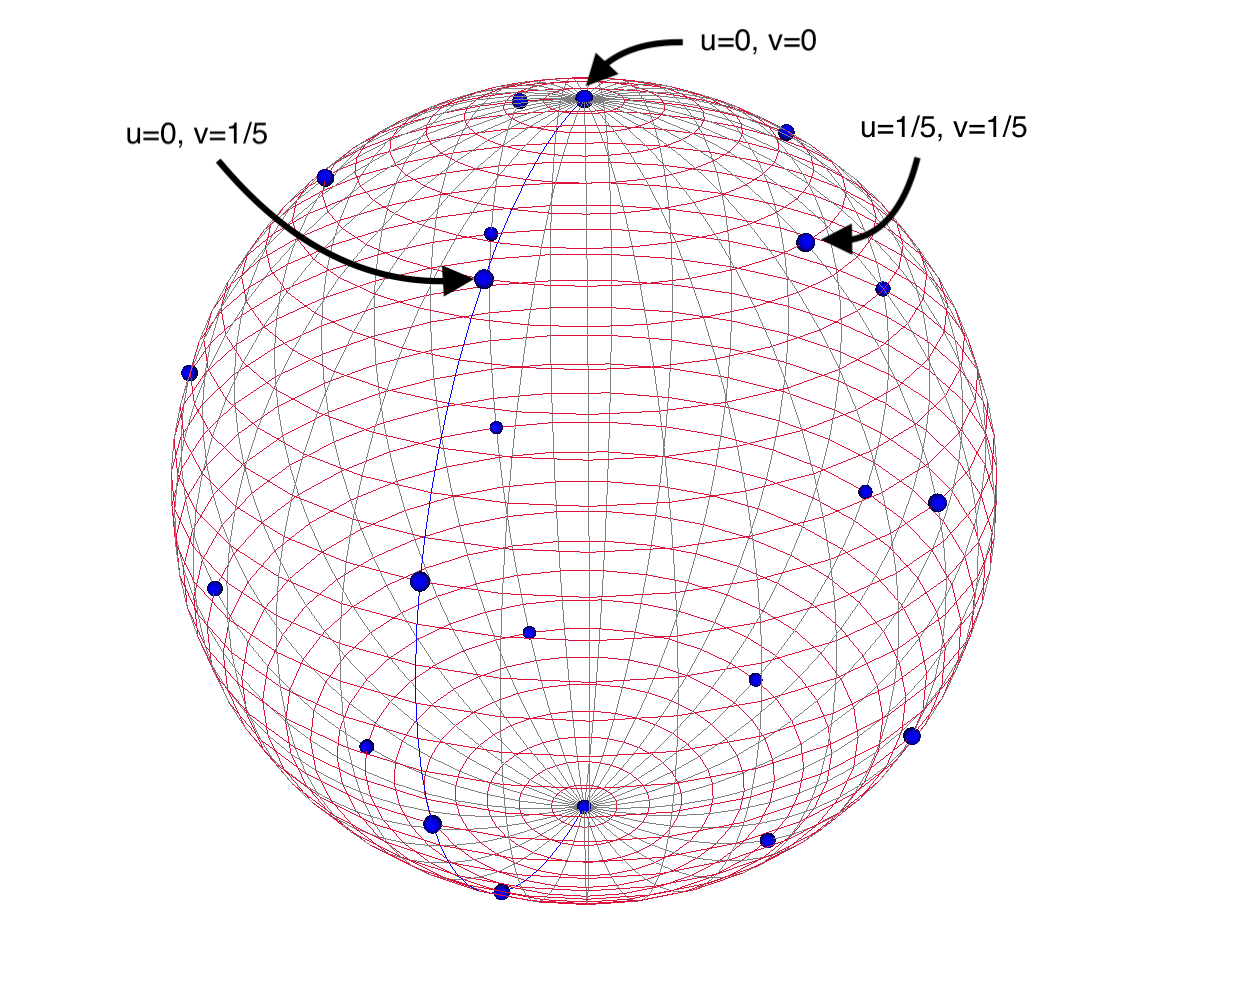
\includegraphics[width=16cm]{sphere_5_5_conti.png}
  \caption{Sphere using Hermite exponentials}
\end{figure}

The usual parametric representation of the unit sphere is
\begin{equation}
  \label{param_sphere}
  \sigma(u,v) = \begin{pmatrix} \cos(2\pi u) \sin(\pi v) \\ \sin(2\pi u) \sin(\pi v)  \\ \cos(\pi v) \end{pmatrix}
\end{equation}

At $u=0, v=0$,
\begin{align*}
  \sigma &= (0, 0, 1) & K &= 1 & n &= (0, 0, 0) & \hat{n} &= (0, 0, 1) \\
  \sigma_1 &= (0, 0, 0) & \sigma_2 &= (0.628, 0, 0) & \sigma_{11} &= (0, 0, 0) & \sigma_{22} &= (0, 0, -0.395) \\
  \sigma_{12}^{can} &= (0, 0.790, 0) & \sigma_{12}^{nor} &= (0,790,0)
\end{align*}

At $u=0, v=0.2$,
\begin{align*}
  \sigma &= (0.588, 0, 0.809) & K &= 1 & n &= (-0.273, 0, -0.375) & \hat{n} &= (-0.588, 0, -0.809) \\
  \sigma_1 &= (0, 0.739, 0) & \sigma_2 &= (0.508, 0, -0.369) & \sigma_{11} &= (-0.928, 0, 0) & \sigma_{22} &= (-0.232, 
  0, -0.319) \\
  \sigma_{12}^{can} &= (0, 0.639, 0) & \sigma_{12}^{nor} &= (0, 0.639, 0)
\end{align*}

Superscript “can” denotes the canonical base $(e_1, e_2, e_3)$ whereas “nor” denote the base made of $(\hat{n}, 
\hat{\sigma_1}, \hat{\sigma_2})$. Note that the latter is indeed a base if none of its components is 0. You may argue 
that at the pole $\sigma_1(0,0)$ is null vector but we will take as definition for the normalized versions of the normal 
and tangents the following

\begin{equation*}
  \hat{n}(u_0, v_0) = \lim_{u \to u_0, v \to v_0} \frac{n}{|n|}(u,v) \qquad \hat{\sigma}_i(u_0, v_0) = \lim_{u \to u_0, 
  v \to v_0} \frac{\sigma_i}{|\sigma_i|}(u,v)
\end{equation*}

Using such definitions one can easily check that for the sphere $\hat{n}(0,0) = (0, 0, 1)$ and $\hat{\sigma}_1(0,0) = 
(0,1,0)$.

\subsection{Hermite polynomial order 1}

The scheme is the extension to surfaces of what V. Uhlmann presented in her article “Hermite snakes with control of 
tangents”. Given that a sphere has closed latitudes and open longitudes, the representation for sphere-like surfaces 
with $M_1$ control points in latitudes and $M_2+1$ in longitudes is 


\begin{align*}
  \sigma(u,v) = \sum_{k=0}^{M_1-1} \sum_{l=0}^{M_2} & \sigma\left(\frac{k}{M_1}, \frac{l}{M_2} \right) \phi_{1 
  per}(M_1u-k)\phi_{1}(M_2v-l) \\
  +\frac{1}{M_2} & \sigma_2\left(\frac{k}{M_1}, \frac{l}{M_2} \right) \phi_{1, per}(M_1u-k)\phi_{2}(M_2v-l) \\
  +\frac{1}{M_1} & \sigma_1\left(\frac{k}{M_1}, \frac{l}{M_2} \right) \phi_{2, per}(M_1u-k)\phi_{1}(M_2v-l) \\
  +\frac{1}{M_1 M_2} & \sigma_{12}\left(\frac{k}{M_1}, \frac{l}{M_2} \right) \phi_{2, per}(M_1u-k)\phi_{2}(M_2v-l) \\
\end{align*}

\begin{wrapfigure}[14]{r}{0.45\textwidth}
  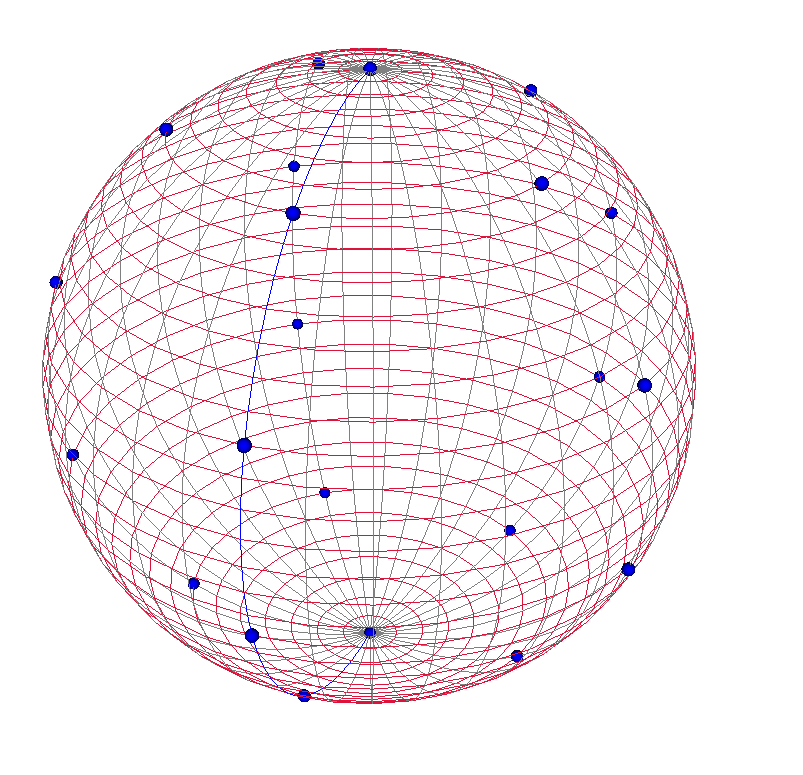
\includegraphics[width=0.45\textwidth]{sphere_5_5_pol.png}
  \caption{Sphere using Hermite polynomials}
\end{wrapfigure}

In the figure on the right a fixed view of the 3D sphere generated by such a scheme for $M_1=5, M_2=5$.  The scheme is 
theoretically not able to reproduce exactly a sphere as cosinus and sinus functions cannot be represented by finite 
polynomials. However as you can see the approximation is very good. In the case of $M_1=5, M_2=5$ the average norm of 
the error at each control point site (30 control points with multiplicity) is $2.24\times 10^{-3}$.


\subsubsection{Twist estimation from $\sigma, \sigma_1, \sigma_2$}

Consider the setting where samples of the surface and the first derivatives are known on a regular grid. In order to 
represent a surface that interpolates this data with a (first-order) Hermite polynomial scheme it remains to specify the 
value of the coefficient (a 3D vector) that goes in front of the term $\phi_{2, per}(M_1.-k)\phi_{2}(M_2.-l)$. As 
mentionned above this term is the scaled first order cross-derivative (or twist vector). Therefore if we can find a way 
to estimate this twist vector from the rest of the data our scheme would be complete. \\

A \emph{naive} way of doing this is to interpolate for example $\sigma_1$ at the different control points on a given 
longitude and compute the derivative of the interpolant at the control points locations. \\

\textbf{Interpolate $\sigma_1$ on each longitude} \mbox{} \\

Interpolating the $M_2+1=6$ available values of each coordinate of $\sigma_1$ for each longitude allows to estimate 
$\sigma_{12}$ at all control points. The average norm error is $9.47\times 10^{-3}$. Example values 

At $u=0, v=0$,
\begin{equation*}
  \text{estimated } \sigma_{12}^{can} = (0, 0.810, 0) \qquad \text{truth } \sigma_{12}^{can} = (0, 0.790, 0) 
\end{equation*}

At $u=0, v=\frac{1}{5}$,
\begin{equation*}
  \text{estimated } \sigma_{12}^{can} = (0, 0.632, 0) \qquad \text{truth } \sigma_{12}^{can} = (0, 0.639, 0) 
\end{equation*}

The estimation is very close to the real value. This is because we have a couple of points but most of all because the 
coordinates of the twist vector are very smooth function in this case! Below is a plot showing the interpolation result 
and it's derivative for the y coordinate of the $\sigma_1(u,.)$ (u=0). 
 
\begin{figure}[h!]
  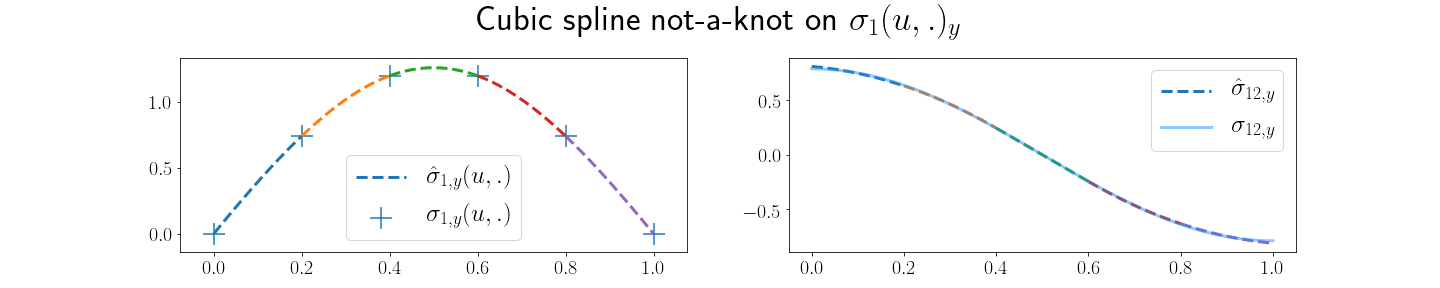
\includegraphics[width=\textwidth]{cubic_sigma_1.png}
  \caption{Cubic spline not-a-knot interpolation of ${\left(\sigma_{1,y}(0,\frac{l}{M_2})\right)}_{l=0}^{M_2}$}
\end{figure}

As detailed by De Boor in “A practical guide to splines” the inteprolation power of this scheme is 
$\mathcal{O}(|\tau|^4)$ (chapter IV p.45) for the function but he doesn't say for the derivative. If of any interest we 
can work out approximation power to the derivative. Estimation works fine for the sphere but it could well be that we 
have a surface where first derivative $\sigma_1$ is $0$ at all control points while the cross-derivative is not. However 
in that case the twist estimated by this technique will obviously be 0. That illustrates one of the many cases where it 
will fail.  \\

\textbf{Interpolate $\sigma_2$ on each latitude} \mbox{} \\

Interpolating the $M_1=5$ available values of each coordinate of $\sigma_2$ for each latitude allows to estimate 
$\sigma_{21}=\sigma_{12}$ at all control points. The average norm error is $0.113$. Example values 

At $u=0, v=\frac{1}{5}$,
\begin{equation*}
  \text{estimated } \sigma_{12}^{can} = (0.085, 0.855, 0) \qquad \text{truth } \sigma_{12}^{can} = (0, 0.639, 0) 
\end{equation*}

At $u=\frac{1}{5}, v=\frac{1}{5}$,
\begin{equation*}
  \text{estimated } \sigma_{12}^{can} = (-0.623, 0.131, 0) \qquad \text{truth } \sigma_{12}^{can} = (-0.608, 0.197, 0) 
\end{equation*}

The error is 10 times higher in that case! First we are using one point less but it also may be that values of 
$\sigma_2$ on a latitude have higher amplitude than $\sigma_1$ on longitude. Below is a representation of the 
interpolation at latitude $v=0.2$. 

\begin{figure}[h!]
  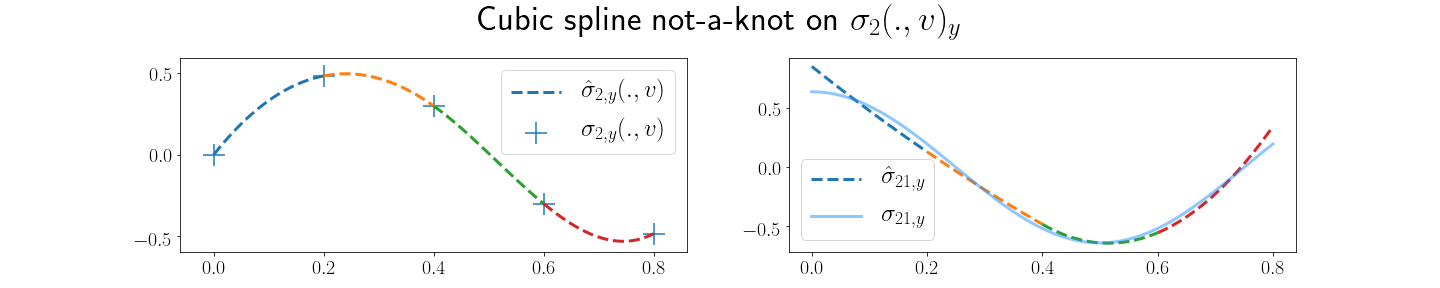
\includegraphics[width=\textwidth]{cubic_sigma_2.png}
  \caption{Cubic spline not-a-knot interpolation of ${\left(\sigma_{2,y}(\frac{k}{M_1}, 0.2)\right)}_{l=0}^{M_1-1}$}
\end{figure}


\subsubsection{Twist estimation from $\sigma, \sigma_1, \sigma_2, K$}

Suppose now that as additional data we have the values of the local curvature (Gaussian curvature) at the control points 
locations. Is there a way to extract the twist vector from that additional information? At a point p on a regular 
surface in $\mathbb{R}^3$, the Gaussian curvature is the determinant of the shape operator that is $K(p) = \text{det } 
S(p)$. It can also be expressed as the ratio of the second fundamental form to the first fundamental form. \textbf{What 
are the minimum requirements on the surface to define these two forms}? In case the surface is the trace of the 
differentiable (definition of differentiable?)  map $\sigma$ and at the point $p$ we have $\sigma_1^2 \sigma_2^2 - 
{(\sigma_1.\sigma_2)}^2 \neq 0$ (i.e $ > 0$) the Gaussian curvature is expressed by

\begin{equation}
  \label{gauss_curv}
  K = \frac{\hat{n}.\sigma_{11} \hat{n}.\sigma_{22} - {\hat{n}.\sigma_{12}}^2}{\sigma_1^2 \sigma_2^2 - 
  {(\sigma_1.\sigma_2)}^2}
\end{equation}

At the point $u=0$, $v=0$ of the sphere with parametrisation (\ref{param_sphere}), $\sigma_1$ is 0 (also at the south 
pole) and thus the above expression cannot be used at this point. At points where determinant of first fundamental form 
is not 0, this formula can be reversed to extract normal component of the twist vector as explained in section 1.1 
(Selesnick's method). \\

In order to inverse formula (\ref{gauss_curv}) to extract $\hat{n}.\sigma_{12}$ one needs to compute somehow 
second-order derivatives $\sigma_{11}, \sigma_{22}$ at control points. Consider the surface on a single patch of the 
form $I_{k,l} = [u_{k}, u_{k+1}]\times[v_l, v_{l+1}]$ the surface is given by

\begin{equation}
  \sigma(u,v) = \begin{bmatrix} f_1(u) \\ f_1(1-u) \\ f_2(u) \\ -f_2(1-u) \end{bmatrix}^T
  \begin{bmatrix}
    \sigma(0,0) & \sigma(0,1) & \sigma_2(0,0) & \sigma_2(0,1) \\
    \sigma(1,0) & \sigma(1,1) & \sigma_2(1,0) & \sigma_2(1,1) \\
    \sigma_1(0,0) & \sigma_1(0,1) & \sigma_{12}(0,0) & \sigma_{12}(0,1) \\
    \sigma_1(1,0) & \sigma_1(1,1) & \sigma_{12}(1,0) & \sigma_{12}(1,1) \\
  \end{bmatrix}
  \begin{bmatrix} f_1(v) \\ f_1(1-v) \\  f_2(v) \\ - f_2(1-v) \end{bmatrix}
\end{equation}


with renoting $u \leftarrow \frac{u-u_k}{\Delta u_k}$, $v \leftarrow \frac{v-v_l}{\Delta v_l}$, $\sigma(u,v) \leftarrow 
\sigma(\frac{u-u_k}{\Delta u_k}, \frac{v-v_l}{\Delta v_l})$ and $f_1$ and $f_2$ being the cubic Hermite polynomials over 
$[0,1]$
\begin{align*}
  f_1(u) &= 1 - 3u^2 + 2u^3 \\
  f_2(u) &= u - 2u^2 + u^3 \\
\end{align*}
  

Let's focus on the control point at $u=0, v=0.2$. Four adjacent patches share this control point as a corner namely 
$I_{0,0}=[0, 0.2]\times[0,0.2]$ (corner (0,1)), $I_{0, 1}=[0, 0.2]\times[0.2, 0.4]$ (corner (0,0)), $I_{4, 0} = [0.8, 
0]\times[0, 0.2]$ (corner (1,1)), $I_{4, 1} = [0.8, 0]\times[0.2, 0.4]$ (corner (1, 0)). For each patch, the second 
derivative at corner $(u,v)$ ($u=0,1, v=0, 1$) is calculated by

\begin{equation}
\sigma_{11}(u,v) =  \begin{bmatrix} f_1^{(2)}(u) \\ f_1^{(2)}(1-u) \\ f_2^{(2)}(u) \\ -f_2^{(2)}(1-u) \end{bmatrix}^T
\begin{bmatrix} \sigma(0,0) f_1(v) + \sigma(0,1) f_1(1-v) \\ \sigma(1,0) f_1(v) + \sigma(1,1) f_1(1-v) \\  \sigma_1(0,0) 
f_1(v) + \sigma_1(0,1) f_1(1-v) \\ \sigma_1(1,0) f_1(v) + \sigma_1(1,1) f_1(1-v) \end{bmatrix}
\end{equation}

where we used the fact that $f_2$ vanishes at 0 and 1. A similar expression holds for calculating $\sigma_{22}$. The 
problem with this calculation is when second derivative $f_1, f_2$ do not have the same value at ends 0 and 1 as is the 
case here. $f_1$ and $f_2$ coincide with $\phi_1$ and $\phi_2$ on $[0,1]$ respectively. 

\begin{figure}[h!]
  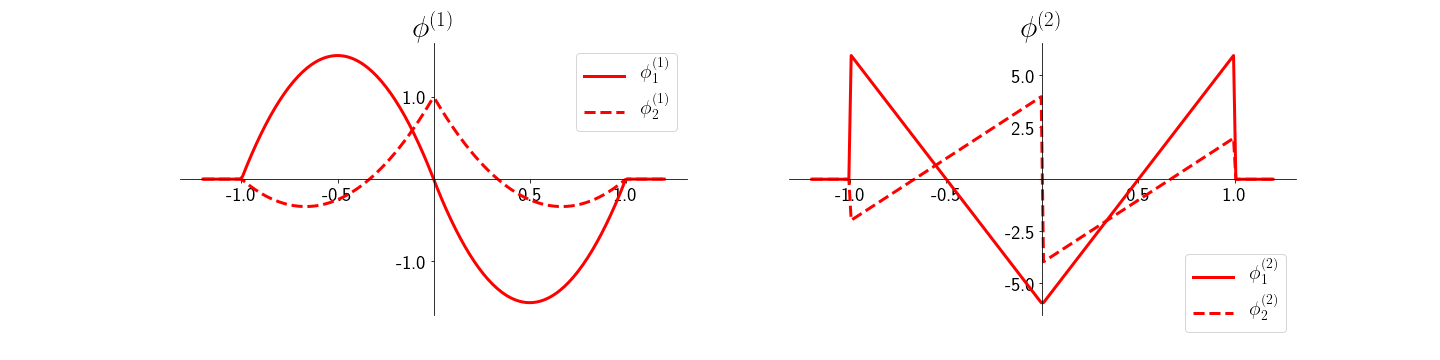
\includegraphics[width=\textwidth]{hermite_order_2.png}
  \caption{First and second derivatives of $\phi_1$ and $\phi_2$ on their domain}
\end{figure}

Let's look at $\sigma_{11}$ calculation at $u=0, v=0.2$ at all four adjacent patches. $\sigma$ in the formulas below is 
the parametric representation of the whole sphere on ${[0,1]}^2$. \\

For $I_{0,0}$,
\begin{equation*}
\sigma_{11}(u,v) =  \begin{bmatrix} -6 \\ 6 \\ -4 \\ -2 \end{bmatrix}^T
\begin{bmatrix} \sigma(0,0.2)  \\ \sigma(0.2,0.2) \\  \frac{1}{M_1} \sigma_1(0,0.2) \\ \frac{1}{M_1} \sigma_1(0.2,0.2) 
\end{bmatrix} = (-1.032, -0.057, 0)
\end{equation*}

For $I_{0,1}$,
\begin{equation*}
\sigma_{11}(u,v) =  \begin{bmatrix} -6 \\ 6 \\ -4 \\ -2 \end{bmatrix}^T
\begin{bmatrix} \sigma(0,0.2)  \\ \sigma(0.2,0.2) \\  \frac{1}{M_1} \sigma_1(0,0.2) \\ \frac{1}{M_1} \sigma_1(0.2,0.2) 
\end{bmatrix} = (-1.032, -0.057, 0)
\end{equation*}


For $I_{4,0}$,
\begin{equation*}
\sigma_{11}(u,v) =  \begin{bmatrix} 6 \\ -6 \\ 2 \\ 4 \end{bmatrix}^T
\begin{bmatrix} \sigma(0.8,0.2)  \\ \sigma(0,0.2) \\  \frac{1}{M_1} \sigma_1(0.8,0.2) \\ \frac{1}{M_1} \sigma_1(0,0.2) 
\end{bmatrix} = (-1.032, +0.057, 0)
\end{equation*}

For $I_{4,1}$,
\begin{equation*}
\sigma_{11}(u,v) =  \begin{bmatrix} 6 \\ -6 \\ 2 \\ 4 \end{bmatrix}^T
\begin{bmatrix} \sigma(0.8,0.2)  \\ \sigma(0,0.2) \\  \frac{1}{M_1} \sigma_1(0.8,0.2) \\ \frac{1}{M_1} \sigma_1(0,0.2) 
\end{bmatrix} = (-1.032, +0.057, 0)
\end{equation*}

One notices the inconsistent estimation of the $y$ coordinate of the $\sigma_{11}$ at $u=0, v=0.2$. As a reminder the 
real value of this vector is $(-0.928, 0, 0)$. As for the $x$ coordinate the estimated value is inexact. \textbf{Why is 
it inexact?}. \\


Once $\sigma_{11}, \sigma_{22}$ are known at control points, it remain to determine the sign in order to compute the 
normal component of the twist. It is chosen to be positive at $u=0, v=0$ and then alternating from one corner to the 
next.  In order to estimate the tangential components of the twist, one needs to estimate derivative with $1$ of 
$|\sigma_1|$ and derivative with $2$ of $|\sigma_2|$ at control points. These are obtained from the slopes at 
interpolation sites of cubic spline interpolation with not-a-knot condition of $|\sigma_1[0, v]|, \ldots, 
|\sigma_1[M_1-1, v]|$ and $|\sigma_2[u, 0]|, \ldots, |\sigma_2[u, M_2]|$ respectively. For the sake of completeness here 
are the four estimations of $\sigma_{22}$ and $\sigma_{12}$ at $u=0, v=0.2$. \\

For $I_{0,0}$,
\begin{equation*}
\sigma_{22}(u,v) = (-0.237, 0, -0.331) \qquad \sigma_{12}(u,v) = (-0.105, 0.632, -0.144)
\end{equation*}

For $I_{0,1}$,
\begin{equation*}
\sigma_{22}(u,v) = (-0.242, 0, -0.328) \qquad \sigma_{12}(u,v) = (0.105, 0.632, 0.144)
\end{equation*}


For $I_{4,0}$,
\begin{equation*}
\sigma_{22}(u,v) = (-0.242, 0, -0.328) \qquad \sigma_{12}(u,v) = (0.105, 0.632, 0.144)
\end{equation*}

For $I_{4,1}$,
\begin{equation*}
\sigma_{22}(u,v) = (-0.237, 0, -0.331) \qquad \sigma_{12}(u,v) = (-0.105, 0.632, -0.144)
\end{equation*}

Again notices inconsistent estimates of second derivatives and hence of the twist vector.


\subsubsection{Twist estimation from $\sigma, \hat{n}, K$}

\subsection{Hermite exponential order 1}

\end{document}
